\documentclass{article}
\usepackage[utf8]{inputenc}
\usepackage[T1]{fontenc} % ASCII-friendly formatting of text
\usepackage{parskip} % no indentation of paragraphs
\usepackage{courier} % for use in lstlistings
\usepackage[margin=1in]{geometry}

\usepackage{float} % for manipulating floats like tables and figures
\restylefloat{table} % allows you to use "H" for hard-fixing table position
\usepackage{graphicx} % for including figures

\usepackage{csquotes} % for block quotes

\usepackage{hyperref}
\newcommand\fnurl[2]{%
  \href{#2}{#1}\footnote{\url{#2}}%
} %for putting hyperlinks in footnotes

\usepackage{listings} % include source code
\usepackage{color} % color source code

\newcommand{\pltlang}{d.o.t.s.} % allows us to just reference the language name with the ``\pltlang'' cmd, so we can change the name later w/o too much hassle

\newcommand{\code}[1]{\texttt{#1}} %sets it up so you can use \code{...} to format text

\definecolor{codegreen}{rgb}{0,0.6,0}
\definecolor{codegray}{rgb}{0.5,0.5,0.5}
\definecolor{codebrown}{rgb}{0.7,0.35,0.25}
\definecolor{backcolor}{rgb}{0.95,0.95,0.92}

\lstdefinestyle{pltStyle}{
  basicstyle=\ttfamily,
  backgroundcolor=\color{backcolor},
  commentstyle=\color{codebrown},
  keywordstyle=\color{blue},
  numberstyle=\tiny\color{codegray},
  stringstyle=\color{codegreen},
  breakatwhitespace=false,
  breaklines=true,
  captionpos=b,
  keepspaces=false,
  numbers=left,
  numbersep=5pt,
  showspaces=false,
  showstringspaces=false,
  showtabs=false,
  tabsize=2
}

\lstdefinelanguage{pltLang}
{
  morekeywords={
    bool,
    true,
    false,
    num,
    string,
    null,
    INF,
    if,
    else,
    for,
    while,
    break,
    in,
    node,
    graph,
    list,
    dict,
    print,
    range,
    def,
    return
  },
  sensitive=true, %keywords are case sensitive
  morecomment=[l]{\#}, % symbol for single-line comment
  morecomment=[s]{\\*}{*\\}, % symbol for multi-line comment
  morestring=[b]" % sets double quote as string indicator
}

\lstset{style=pltStyle, columns=flexible}

\title{d.o.t.s. \\ A graph language.}
\author{Hosanna Fuller (hjf2106) --- Manager\\
Rachel Gordon (rcg2130) --- Language Guru\\
Yumeng Liao (yl2908) --- Tester\\
Adam Incera (aji2112) --- System Architect}
\date{September 2015}

\begin{document}

\maketitle

\tableofcontents
\newpage

\section{Introduction and Motivation}
Graphs are a  powerful and versatile data structure used across many languages to help visually organize and manipulate data. Many languages do not provide out-of-the-box  support for data structures and methods useful in solving graph problems. Because of this, programmers end up spending unnecessary time and energy implementing these critical structures themselves. As a result, graph implementations often widely vary in efficiency and modularity. The goal of \pltlang\ is to provide an out-of-the-box graph framework so that users can focus on creating the algorithms needed to solve their problems, rather than getting bogged down in implementation issues. With d.o.t.s., users can comprehensively solve a wide variety of graph-based problems. Some example problems include:  expressing network relationships such as a series of interconnected routers with edge costs, representing decision trees in probability, and running analyses on propositional models. 

\section{Language Design and Syntax}

The strict typing and control flow in \pltlang\ is reminiscent of C and Java, but overall the language is intended to be used more as a scripting language, where the user builds their graphs quickly using the intuitive node and edge operators and then performs operations on the structures. 

The \pltlang\ compiler compiles code written in \pltlang\ into C, and then uses the GNU C Compiler to build binary executables.

{\emph{Note:}} In the following sections, the word ``graph'' is sometimes used to denote a data structure and sometimes to denote the abstract structure from computer science and mathematics:

\begin{displayquote}
A graph data structure consists of a finite (and possibly mutable) set of nodes or vertices, together with a set of ordered pairs of these nodes (or, in some cases, a set of unordered pairs). These pairs are known as edges or arcs. As in mathematics, an edge (x,y) is said to point or go from x to y. The nodes may be part of the graph structure, or may be external entities represented by integer indices or references.

A graph data structure may also associate to each edge some edge value, such as a symbolic label or a numeric attribute (cost, capacity, length, etc.). \fnurl{}{https://en.wikipedia.org/wiki/Graph_(abstract_data_type)}
\end{displayquote}

For the sake of clarity, from this point forward we will refer to the language-specific data structure using the lowercase ``graph'' and the mathematical concept using the uppercase ``Graph.''

\subsection{Comments}

\begin{table}[H]
\centering
\begin{tabular}{| p{.75in} | p{2in} |}
\hline
Syntax & Comment Style \\
\hline
\textbackslash*

$\quad$\emph{code} 

*\textbackslash & multi-line comment \\
\hline
\# & single-line comment \\
\hline
\end{tabular}
\caption{Comment Styles}
\label{tbl:comments}
\end{table}

\subsection{Built-in Data Types}

\pltlang\ comes with three basic types: \code{num, bool}, and \code{string}. Each of these basic types can be used as raw values with no prior declaration of variables or can be assigned as the values of variables. \pltlang\ also provides two built-in data types, \code{node} and \code{graph}, which provide the basis for algorithms written in \pltlang{} The built-in collections are: \code{list}, and \code{dict}. \pltlang\ is a strictly-typed language, meaning that the types of all variables must be declared at the same time that the variable is declared.

In addition to these data types, \pltlang\ also includes the value \code{null}, which represents the absence of value for any data type.

\begin{table}[H]
\centering
\begin{tabular}{| p{.75in} | p{2in} |}
\hline
Data Type & Fields \\
\hline
num & \\
string & \\
bool & \\
list &  \\
dict &  \\
node & value, in, out \\
graph & vertices \\
\hline
\end{tabular}
\caption{Built-in Data Types}
\label{tbl:data_types}
\end{table}

\subsection{Nums and Strings}

\begin{table}[H]
\centering
\begin{tabular}{| p{.8in} | p{1in} | p{1.5in} | p{2.5in} | }
\hline
Category & Data Type & Operator & Explanation \\
\hline
comparison & num, string & <, >, <=, >=, !=, == & Operate in the same way as languages such as C/C++, with the exception that string equality compares the \emph{value} contained in the string. \\
\hline
computation & num & +, -, *, /, \% & Operate in the same way as languages such as C/C++. \\
\hline
concatenation & string & + & String concatenation operator \\
\hline
\end{tabular}
\caption{Num and String Operators}
\label{tbl:comp_ops}
\end{table}

In addition to literal \code{num} values, \pltlang\ provides an infinity value for the \code{num} type: \code{INF}. The operators perform a little differently for these values. As the primary use of infinity in graph problems is to define edge weight and not to perform mathematical calculations, the computation operators cause an exception whenever infinity is an operand. 

For comparison operators, \code{INF} is greater than all non-null non-infinity values and equal to other infinity values. Defining the comparison operators for \code{INF} values allows them to be used as valid edge weights, which can be useful for graph problems.


\begin{lstlisting}[language=pltLang, caption=Demonstration of ``num'' and ``string'' types., label=lst:num-str]
num x = 12.0, y = 6 * 2.0, z = 6.5, i = INF;
x == y;   # returns true
y < z;    # returns false

y > INF;  # returns false
num h = 2 + i; # exception


string z = "Hello" + " " + "World";    # z = "Hello World"
string a = "cat", b = "bear";
a < b;    # returns true;


\end{lstlisting}

\subsection{Node and Graph Objects}

The data types which underpin \pltlang\ and give it its advantage in the Graph domain over languages such as C are \code{node} and \code{graph}. From the get-go any programmer using \pltlang\ can use these data types to quickly build Graphs without the need to waste time creating these data structures from scratch.

A \code{node} object represents a single vertex in a Graph, whereas a \code{graph} object represents a collection of graphs (which can be empty). \emph{Note}: A node is a graph, but a graph is not a node.\\

Recursive definition of graph objects:
\begin{itemize}
\item An empty graph is a graph.
\item A node is a graph.
\item A graph added to a graph is a graph.\\
\end{itemize}

A graph contains only the field \code{vertices}, which is a list of all node objects contained within the graph. 

A node contains the fields \code{value, in, out}. Internally, a node uniquely identified by an id number set by the compiler, but this distinction is invisible to the programmer. The \code{value} field is a string object, and simply represents some value that the node contains. One possible use of the value field is to allow users to assign a more semantic meaning to nodes (ex. setting the value to the name of a city). The \code{in} field is a dict mapping nodes that the current node has edges into to weights. Similarly, the \code{out} field is a dict mapping nodes that have edges into the current node to weights. The keys of the two dicts are nodes. An example of accessing the \code{in} and \code{out} dicts of a node can be seen in Listing \ref{lst:node-ops}.

Since node has an \emph{is-a} relationship with graph, it also contains a \code{vertices} field, but this is set upon declaration to contain only the node itself, and cannot be altered by the user.

Nodes can be declared in two different ways. In the first, the variable can be simply be declared with the \code{node} keyword and a variable name. This creates a basic node with an empty value, in\_list, and out\_list. In the second manner, a node can be declared by giving it an initial value inside parentheses after the variable name (as seen in line 11 of Listing \ref{lst:node-graph-dec}). Alternatively, a declared variable can be initialized with the assignment operator ``='' to any object of the type \code{node}.

As with all other types, graphs can be assigned at the same time as declaration or assigned later. A graph can be assigned any expression that evaluates to something of the type \code{graph}. There is also a special graph-creation syntax that can \emph{only} be used at declaration time of a graph object  (as seen in lines 6-9 of Listing \ref{lst:node-graph-dec}). This special syntax consists of a comma-separated list of nodes and/or node operations (an example of this syntax can be found in lines 26-32 of Listing \ref{lst:node-ops}). Each node referenced in this type of assignment must have been previously declared. \\

\begin{lstlisting}[language=pltLang, caption=Declaration of ``node'' and ``graph'' objects., label=lst:node-graph-dec]
node x;
node y("nyc");

graph g1;
graph g2 = g1;
graph g3 = { 
    x,
    y
};  # special graph assignment syntax only available at declaration time

\end{lstlisting}

\subsection{Collections -- Dicts and Lists}

Lists are declared using the keyword \code{list} and an indicator of the type of the list, as all objects in a list must be of the same type. Lists can be assigned by putting a comma-separated list of objects inside brackets, or can be filled using list functions.

Dictionary objects in \pltlang\ represent mappings from objects to objects; a key can be any type for which the comparison operator ``\code{==}'' has been defined, and all keys in a given dict must be of the same type. Similarly, all values in a given dict must be of the same type. Dict objects are declared in a similar manner to lists, using the keyword \code{dict} and an indicator of the type that the dict maps from and to. Dicts can be assigned by putting a comma-separated list of \code{key:value} pairs inside curly braces.

\begin{table}[H]
\centering
\begin{tabular}{| p{1.5in} | p{2in} | p{2.25in} | }
\hline
Operation & Syntax & Explanation \\
\hline
\underline{List Ops} & & \\
& & \\
random access & \code{\emph{listVar}[\emph{index}]} & returns the element at the index \\
contains element & \code{\emph{valueVar} in \emph{listVar}} & returns \code{true} if \emph{value} appears in \emph{listVar}, else returns \code{false}  \\
enqueue & \code{\emph{listvar}.enqueue(\emph{elemVar})} & appends the given variable to the end of the list \\
dequeue & \code{\emph{listvar}.dequeue()} & removes and returns the first element of the list \\
element deletion & \code{\emph{listvar}.remove(\emph{value})} & removes first instance of \emph{value} in the list. Returns \code{true} if an element was removed, else \code{false}. \\
\hline
\underline{Dict Ops} & & \\
& & \\
value access & \code{\emph{dictVar}[\emph{key}]} & returns the value at the given key. \emph{key} can be a raw value or variable. \\
contains key & \code{\emph{keyVar} in \emph{dictVar}} & returns \code{true} if the key \emph{keyVar} is in the dict \emph{dictVar} \\
value assignment & \code{\emph{dictVar}[\emph{key}] = \emph{newValue}} & if \emph{key} already exists in the dict, overrides the old value with \emph{newValue}, else adds the (\emph{key,newValue}) pair to the dict. \\
element deletion & \code{\emph{dictVar}.remove(\emph{keyVal})} & removes the (key, value) pair with key \emph{keyVal} from the dict.\\
\hline
\end{tabular}
\caption{List and Dict Operations}
\label{tbl:dict-list-ops}
\end{table}

\begin{lstlisting}[language=pltLang, caption=Declaration of ``list'' and ``dict'' types., label=lst:list-dict-dec]
list<num> numList = [1, 2, 3];
2 in numList; # returns true

list<string> strList = ["Hello"];
strList.enqueue(" ");
strList.enqueue("World"); # strList now equals ["Hello", " ", "World"];
string s = strList.dequeue(); # strList = ["Hello", " "] and s = "World"

dict<string, num> numDict = {"one" : 1, "two" : 2, "three" : 3};
"three" in numDict; # returns true
bool success = numDict.remove("three"); 
\* Now:
    numDict = {"one" : 1, "two" : 2}
    success = true
 *\

dict<node, num> cityRankings;
node x("chicago");
cityRankings[x] = 2;
node y("seattle");
cityRankings[y] = 1;

\end{lstlisting}



\subsection{Node Operators}

The node operators outlined in Table \ref{tbl:node-ops} are all binary operators which take a node object on the left-hand and right-hand sides of the operator.

\begin{table}[H]
\centering
\begin{tabular}{| p{1.5in} | p{2.75in} |}
\hline
Operator & Explanation \\
\hline
\texttt{-{}-} & Add undirected edge with no weights between the 2 \\
\hline
\texttt{-{}-}> & Add directed edge from left node to right node with no weight \\
\hline
\texttt{-{}-}[\emph{num}] & Add an undirected edge between 2 nodes with weight \emph{num} in both directions \\
\hline
\texttt{-{}-}>[\emph{num}] & Add a directed edge from the left node to the right node with weight \emph{num} \\
\hline
[\emph{num}]\texttt{-{}-}[\emph{num}] & Add edge from left to right with the weight in the right set of brackets, and an edge from right to left with the weight in the left set of brackets \\
\hline
== & Returns whether the internal ids of 2 nodes match \\
\hline
!= & Returns whether the internal ids of 2 nodes do not match \\
\hline
\end{tabular}
\caption{Node Operators}
\label{tbl:node-ops}
\end{table}

\begin{figure}[H]
\centering
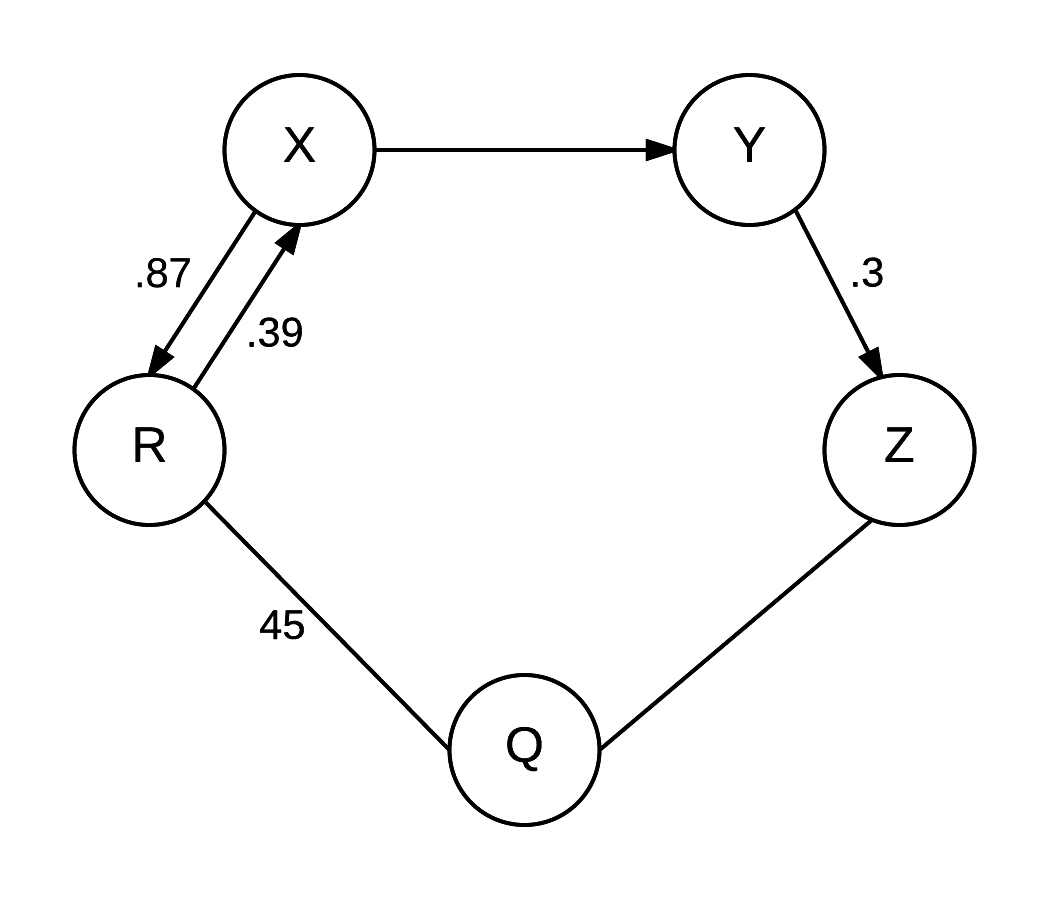
\includegraphics{graphs/node_operators_example.png}
\caption{Example Graph showing nodes with different weights and edges.}
\label{fig:node-ops}
\end{figure}


\begin{lstlisting}[language=pltLang, caption=Shows the use of node operators that creates the graph in Figure \ref{fig:node_ops}., label=lst:node-ops]
node X, Y, Z, Q, R;

X --> Y;
Y -->[.3] Z;
Z -- Q;
Q --[45] R;
R [.87]--[.39] X;

R == Q;    # returns false
R != Q;   # returns true

\* accessing edge lists: *\
X.out[Y]; # == null
Y.out[Z]; # == .3
R.in[X]; # == .87

node alt = Z;
Y.out[alt] == Y.out[Z]; # returns true

\* Alternate Graph Creation:
 * adds the nodes to the graph G, while
 * at the same time it adds edges and weights
 * between the nodes
 *\
node x, y, z, q, r;
graph G = {
    x --> y,
    y -->[.3] z,
    z -- q,
    q --[45] r,
    r [.87]--[.39] x
};
    

\end{lstlisting}

\subsection{Graph Operators}

The graph operators outlined in Table \ref{tbl:graph-ops} are all binary operators which take a graph object on the left-hand and right-hand sides of the operator.

\begin{table}[H]
\centering
\begin{tabular}{| p{1.5in} | p{2.75in} |}
\hline
Operator & Explanation \\
\hline
+ & Returns a graph that contains all of the graphs in the left-hand and right-hand graph \\
\hline
+= & Adds the graph on the right-hand side of the operator to the graph on the left-hand side. \\
\hline
-= & Removes the graph on the right-hand side of the operator from the graph on the left-hand side. \\
\hline
== & Returns whether the two graphs contain the same nodes. \\
\hline
\end{tabular}
\caption{Graph Operators}
\label{tbl:graph-ops}
\end{table}

\begin{figure}[H]
\centering
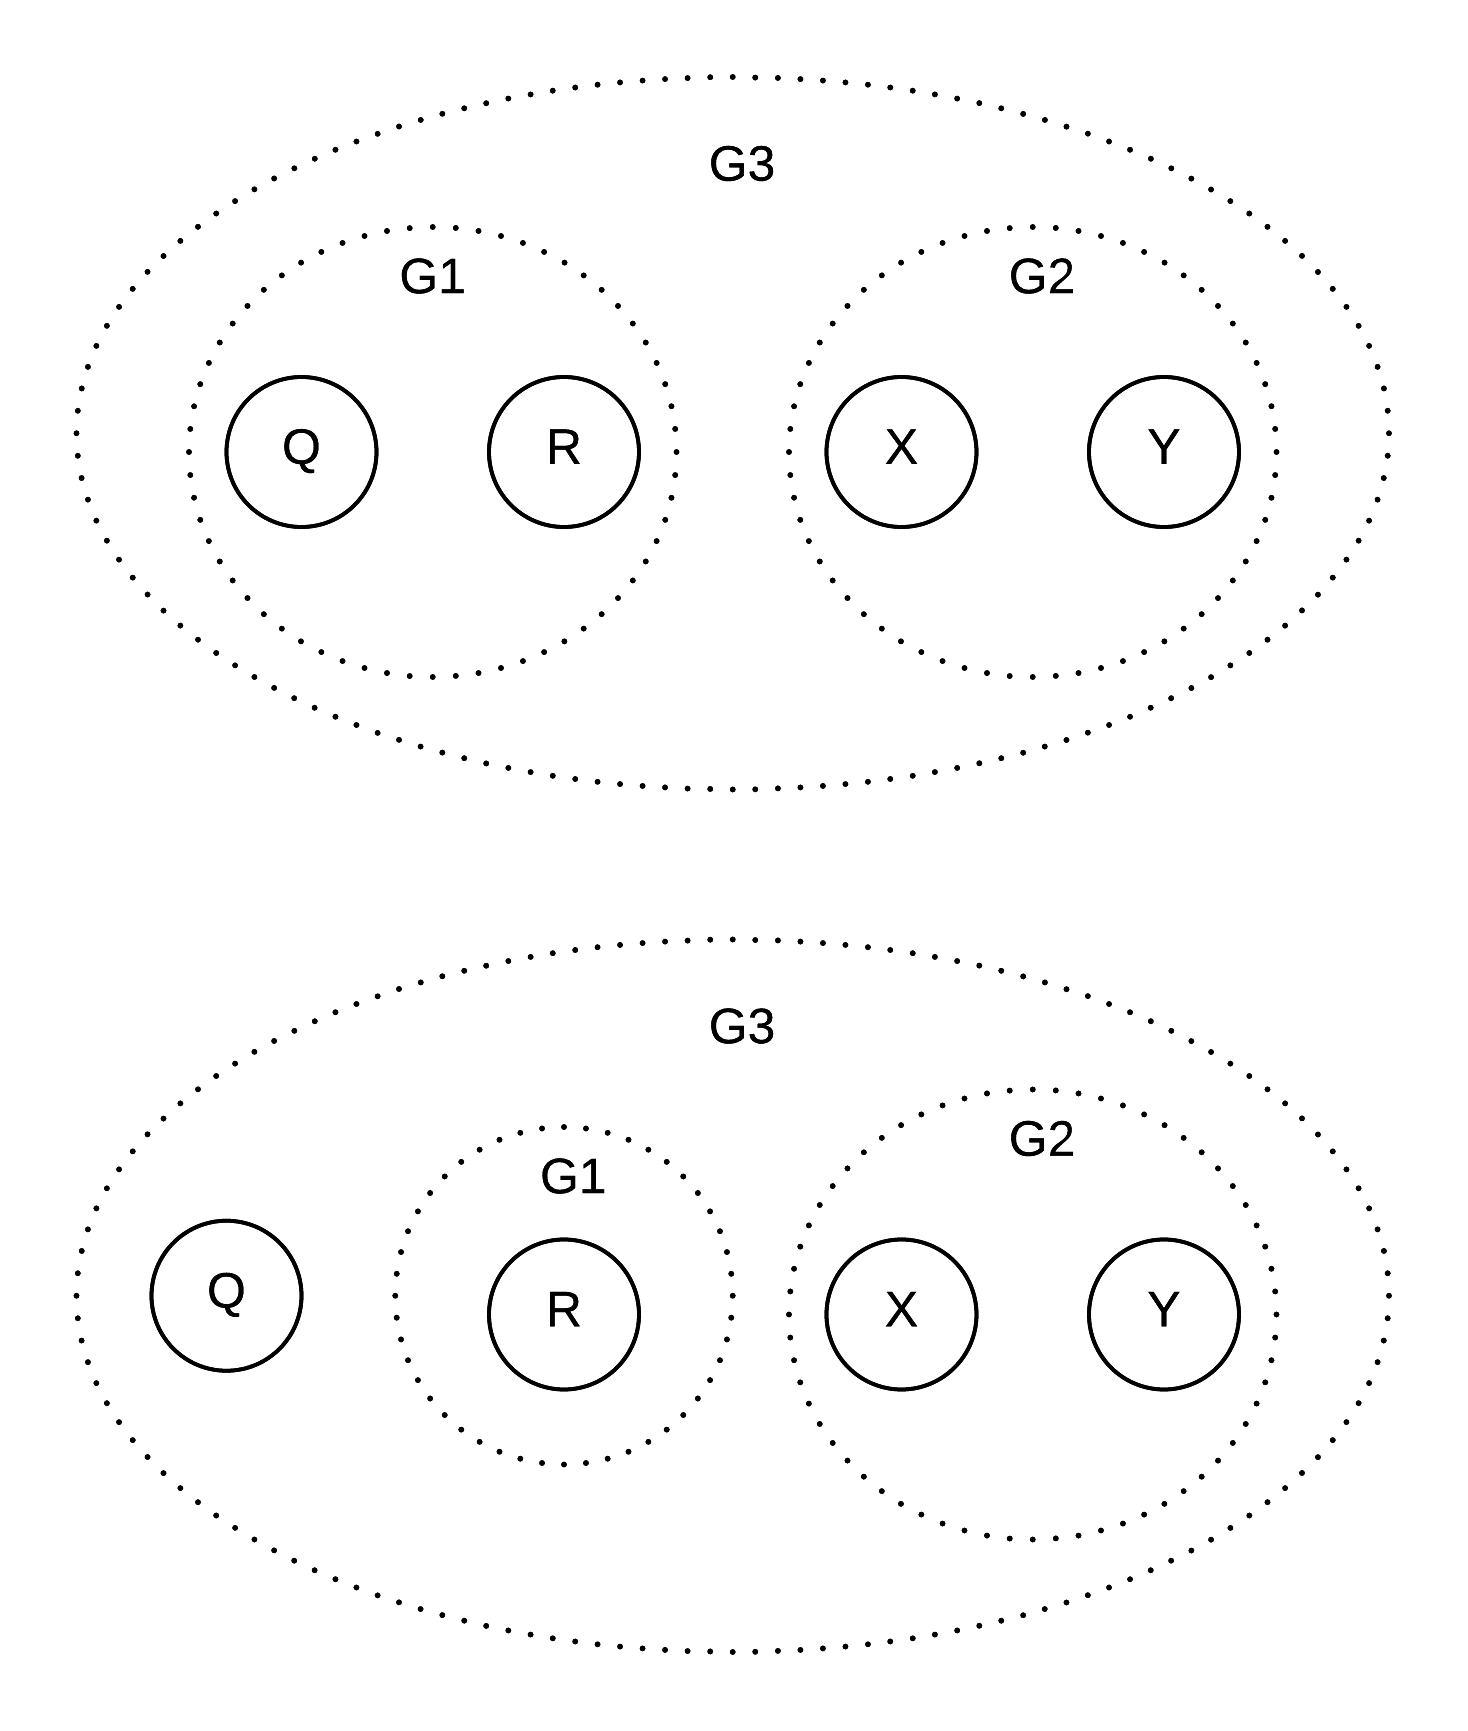
\includegraphics{graphs/graph_ops_example.png}
\caption{Example showing graphs and graph nesting. The bottom graph is the result of removing the node ``Q'' from the graph G1.}
\label{fig:graph-ops}
\end{figure}

\begin{lstlisting}[language=pltLang, caption=Shows the use of graph operators that creates the top graph in Figure \ref{fig:graph-ops} and then alters it to the bottom graph shown., label=lst:graph-ops]
node X, Y, Q, R;
graph G1, G2, G3;
G2 = X + Y;
G1 = Q;
G1 += R;
G3 = G1 + G2;  # result is the top graph
G1 -= Q;  # result is now the bottom graph

\end{lstlisting}

\subsection{Built-in Functions}

\begin{table}[H]
\centering
\begin{tabular}{| p{2.75in} | p{2.5in} |}
\hline
Syntax & Explanation \\
\hline
print(x, ...) & prints to standard output the string representation of a list of comma-separated values or variables. \\
\hline
range(\emph{int\_lower}, \emph{int\_upper}) & returns a list of the integers from \emph{int\_lower} to \emph{int\_upper}, inclusive. The first argument can be ommitted, in which case 0 will be used as the default value of \emph{int\_lower}. The data type of both arguments must be int. \\
\hline
len(\emph{iterable\_var}) & returns the length of the iterable variable \\
\hline
isEmpty(\emph{iterable\_var}) & returns \code{len(\emph{iterable\_var}) $>$ 0} \\
\hline
max(\emph{iterable\_var}) & Uses the ``\code{>}'' operator for detrmining values; if ``\code{>}'' is undefined for the object, returns \code{null}. For lists, returns the element with greatest value. For dicts, returns the key of (key,value) pair with the greatest value. \\
\hline
min(\emph{iterable\_var}) & Uses the ``\code{<}'' operator for detrmining values; if ``\code{<}'' is undefined for the object, returns \code{null}. For lists, returns the element with lowest value. For dicts, returns the key of (key,value) pair with the lowest value. \\
\hline
\end{tabular}
\caption{Built-in Functions}
\label{tbl:functs}
\end{table}

\begin{lstlisting}[language=pltLang, caption=Shows the use of built-in functions., label=lst:functs]
list<int> x = range(1, 3);
list<int> y = range(3);

print("x: ", x, "\ny:", y);
\* prints out -->
  x: [1, 2, 3]
  y: [0, 1, 2, 3]
*\

list<string> q = ["foo", "fah"];
len(q); # returns 2
isEmpty(q); # returns false

dict<string, num> cityVals = {"chicago" : 2, "seattle" : 1, "nyc" : -8};
max(cityVals); # returns "chicago"
min(cityVals); # returns "nyc"

\end{lstlisting}

\subsection{Control Flow}

As Section \ref{sec:code} includes example usage for each of the different types of control statements, this section omits a separate demonstration of their use.

\begin{table}[H]
\centering
\begin{tabular}{| p{3in} | p{2.75in} |}
\hline
& Explanation \\
\hline
if \emph{condition} \{ 

$\quad$ \textbackslash* code *\textbackslash 

\}

else \{

$\quad$ \textbackslash* code *\textbackslash  

\}

& if else statement \\
\hline
while \emph{condition} \{ 

$\quad$ \textbackslash* code *\textbackslash

\} & while loop \\
\hline
for \emph{var\_name} in \emph{iterable\_var} \{

$\quad$ \textbackslash* code *\textbackslash

\} & Iterates through all the elements of the iterable variable, assigning the current element to \emph{var\_name}. \\
&\\
example:

for \emph{node\_var} in \emph{graph\_var} \{

$\quad$ \textbackslash* code *\textbackslash 

\} & Iterates through all the nodes contained in \emph{graph\_var}, assigning the current node to the variable \emph{node\_var}. \\
\hline
def \emph{return\_type} \emph{funct\_name} (\emph{param1\_type} \emph{param1\_name}, ...) \{

$\quad$ \textbackslash* code *\textbackslash

\}

& function declaration \\
\hline
\end{tabular}
\caption{Control-flow Syntax}
\label{tbl:control}
\end{table}

\section{Sample Code}
\label{sec:code}

In this section, we demonstrate how two simple path-searching algorithms can be implemented using \pltlang's syntax. The end-goal of our project is to be able to implement more complex algorithms. But for the purposes of demonstration, we chose to show Dijkstra's Algorithm (Listing \ref{lst:dijkstras}) and the Breadth-First Search algorithm (Listing \ref{lst:bfs}), as their implementation make use of each collection type and control-flow statement. 


\lstinputlisting[language=pltlang, label={lst:dijkstras}, caption=Dijkstra's Algorithm]{dijkstras.dots}

\lstinputlisting[language=pltlang, label={lst:bfs}, caption=Breadth-First Search Algorithm]{bfs.dots}

Now that we have defined the \code{bfs} and \code{dijkstra} functions, we can use them to find shortest paths in an actual instance of a graph.

\begin{figure}[H]
\centering
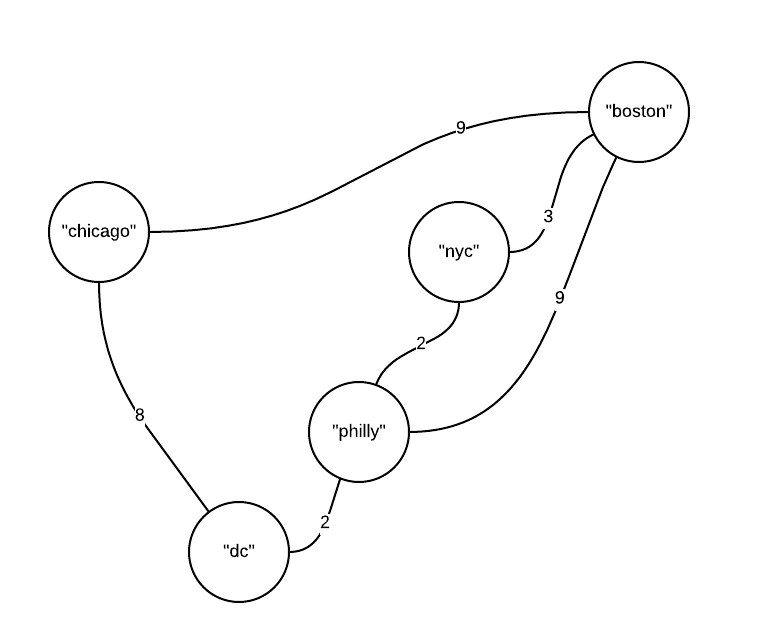
\includegraphics[width=0.65\textwidth]{graphs/example_city_graph.png}
\caption{Visual representation of graph created in Listing \ref{lst:path-search}.}
\label{fig:node_ops}
\end{figure}


\begin{lstlisting}[language=pltLang, caption=Using user-defined functions., label=lst:path-search]
\* Graph set-up *\
node x("dc"), y("chicago"), z("philly"), q("nyc"), r("boston");

graph g1 = {
    x --[2] z;
    z --[2] q;
    q --[3] r;
    z --[9] r;
    x --[8] y;
    y --[9] r;
};
\* end Graph set-up *\

# find the min costs from "philly" to all other cities:
dict<node, num> min_costs = dijkstra(g1, z);

# find path with minimum number of hops from "philly" to "chicago":
list<node> min_path = bfs(g1, z, y);


\end{lstlisting}

\end{document}
